\section{Frequnzverhalten analoger LTI-Systeme}

\begin{minipage}[c]{0.5\columnwidth}
    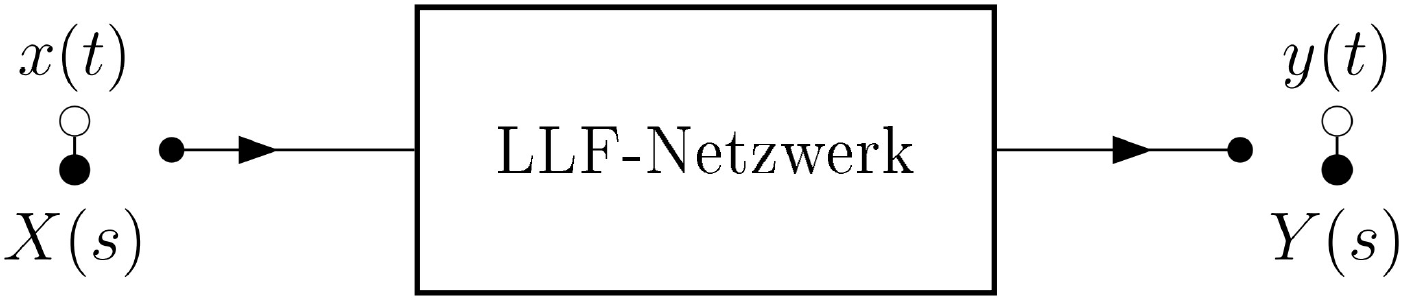
\includegraphics[width=\columnwidth]{images/llf_netzwerk.png}
\end{minipage}
\hfill
\begin{minipage}[c]{0.48\columnwidth}
    Die Betrachtungen beschränken sich auf \textbf{zeitinvariante} LLF-Netzwerke (lineare Netzwerke mit konzentrierten Elementen)
\end{minipage}




\subsection{Zusammenhang Frequenzgang -- UTF}

Alle LTI-Systeme lassen sich mit einer Differntialfleichung der folgenden Form beschreiben:
$$ \scriptstyle{a_n \frac{\diff^n y}{\diff t^n} + a_{n-1} \frac{\diff^{n-1} y}{\diff t^{n-1}} + \cdots + a_1 \frac{\diff y}{\diff t} + a_0 y =
    b_m \frac{\diff^m x}{\diff t^m} + b_{m-1} \frac{\diff^{m-1} x}{\diff t^{m-1}} + \cdots + b_1 \frac{\diff x}{\diff t} + b_0 x } $$

Die Laplace-Transformierte der DGL hat die Form 
$$ \boxed{ H(s) = \frac{Y(s)}{X(s)} = \frac{b_m s^m + b_{m-1} s^{m-1} + \cdots + b_1 s + b_0}
{a_n s^n + a_{n-1} s^{n-1} + \cdots + a_1 s + a_0}  = \frac{N(s)}{D(s)} }$$

\begin{tabular}{ll c ll}
    $N(s)$ & Zählerpolynom mit konstanten, reelen Koeffizienten \\
    $D(s)$ & Nennerpolynom mit konstanten, reelen Koeffizienten \\
    $x(t)$ & Eingangssignal \\
    $y(t)$ & Ausgangssignal \\
\end{tabular}

\vspace{0.2cm}

Die Wurzeln der Gleichung $N(s) = 0$ ergeben $m$ endliche Nullstellen; die Wurzeln von $D(s) = 0$ ergeben $n$ Pole des Systems.
\textbf{Aus Stabilitätsgründen müssen alle Pole in der linken Halbebene (LHE) liegen!}


\subsubsection{Praktische Schreibweise für Pol-/Nullstellen}

Um die Pole bzw. Nullstellen des Systems direkt ablesen zu können, wird $H(s)$ faktorisiert. \textrightarrow Die UTF $H(s)$ ist durch
die Pole, Nullstellen und den Faktor K \textbf{vollständig bestimmt}!

$$ H(s) = \underbrace{\frac{b_m}{a_m}}_{K} \cdot \frac{\prod\limits_{i=1}^m (s - z_i)}{\prod\limits_{j=1}^n (s - p_j)} $$


Da die Wurzeln von Polynomen mit reellen Koeffizienten entweder reell oder konjugiert-komplexe Paare auftreten, ist es meistens
sinnvoll, die Systemfunktionen als Produkt von Faktoren 1. und 2. Ordnung mit reelen Koeffizienten darzustellen.

$$ H(s) = \underbrace{\frac{b_m}{a_m}}_{K} \cdot 
    \frac{\prod\limits_{i=1}^r (\cbl{s^2 + 2 \sigma_{zi} s + \omega_{zi}^2}) \prod\limits_{i=2r+1}^m (\cgn{s - z_i})}
    {\prod\limits_{j=1}^t (\cor{s^2 + 2 \sigma_{pj} s + \omega_{pj}^2}) \prod\limits_{j=2t+1}^n (\cvt{s - p_j})} $$


% colors must be updated --> better visibility
\textbf{Legende:}
\begin{itemize}
    \item \cbl{Beschreibt komplex-konjugierte Nullstellen in der LHE} 
    \item \cgn{Beschreibt reelle Nullstellen in der LHE}
    \item \cor{Beschreibt komplex-konjugierte Polein der LHE} 
    \item \cvt{Beschreibt reelle Pole in der LHE} 
\end{itemize}

\vspace{0.2cm}

Alternativ kann $H(s)$ mittels \textbf{Polfrequenzen} und \textbf{Polgüten} beschrieben werden:
$$ H(s) = \underbrace{\frac{b_m}{a_m}}_{K} \cdot 
    \frac{\prod\limits_{i=1}^r (s^2 + \frac{\omega_{zi}}{q_{zi}} s + \omega_{zi}^2) \prod\limits_{i=2r+1}^m (s - z_i)}
    {\prod\limits_{j=1}^t (s^2 +\frac{\omega_{pj}}{q_{pj}} s + \omega_{pj}^2) \prod\limits_{j=2t+1}^n (s - p_j)} $$

\begin{tabular}{ll c ll}
    $\omega_{pj}$   & Polstellenfrequenzen & 
    $\omega_{zi}$   & Nullstellenfrequenzen \\
    $q_{pj}$        & Polstellengüten & 
    $q_{zi}$        & Nullstellengüten
\end{tabular}


\subsection{Pol- und Nulstellendiagramme}

\begin{minipage}[c]{0.5\columnwidth}
    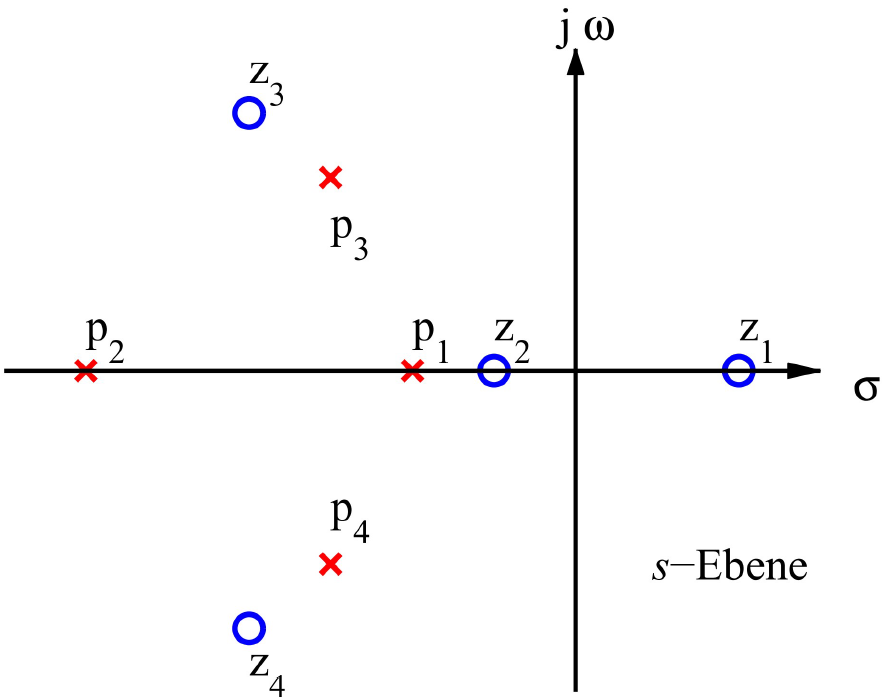
\includegraphics[width=\columnwidth]{images/pol_nullstellen_diagramm.png}
\end{minipage}
\hfill
\begin{minipage}[c]{0.48\columnwidth}
    Werden die Pole und Nullstellen in der komplexen Zahlenebene dargestellt, so spricht man von einem Pol-/Nullstell-Diagramm \\
    In Mathlab erzeugt der Befehl 'pzmap' einen solchen Plot \\ % Schriftart von 'pzmap' ändern?

    \begin{tabular}{ll}
        Pole    & Kreuze \\
        NS      & Kreise \\
    \end{tabular}
\end{minipage}


\subsection{Pole in der komplexen Zahlenebene}{214}

\example{Polynom 2. Ordnung mit komplex-konjugierten Polen}

\begin{minipage}[c]{0.45\columnwidth}
    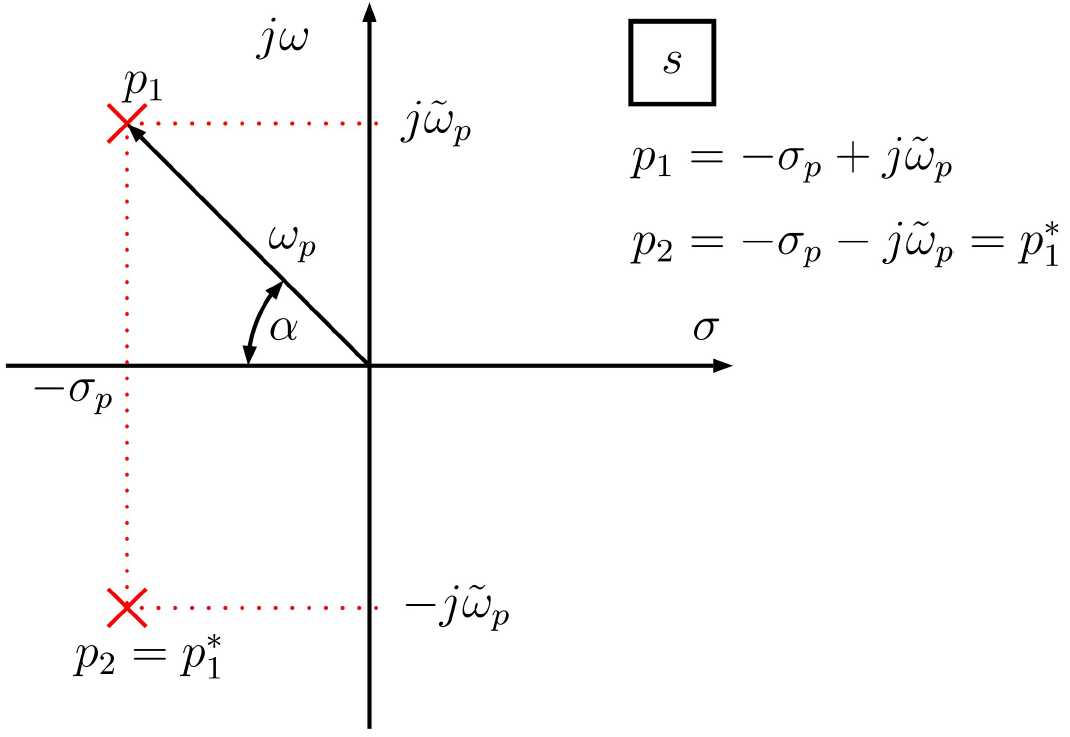
\includegraphics[width=\columnwidth]{images/beispiel_pol_nullstellen_diagramm.png}
\end{minipage}
\hfill
\begin{minipage}[c]{0.48\columnwidth}
    $$(s - p_1) \cdot (s -p_2) = s^2 + 2 \sigma_p s + (\sigma_p^2 + \tilde{\omega_p^2}) $$
    $$ \boxed{ \omega_p = \sqrt{\sigma_p^2 + \tilde{\omega_p^2}}} $$
    $$ \boxed{ q_p = \frac{\omega_p}{2 \sigma_p} = \frac{1}{2 \cdot \cos(\alpha)}} $$
\end{minipage}

\begin{tabular}{ll}
    $\omega_p$  & Polfrequenz \textrightarrow Entspricht Abstand des Pols vom Ursprung \\
    $q_p$       & Polgüte \\
\end{tabular}

\vspace{0.2cm}
\textbf{\myul{Grenzfälle}} \\
\begin{tabular}{lll}
    $\sigma_p = \omega_p$   & Doppelpol auf neg. reeller Achse  & \textrightarrow $q_p = \frac{1}{2}$ \\
    $\sigma_p = 0$          & Polpar auf imaginärer Achse       & \textrightarrow $q_p = \infty$
\end{tabular}


\subsubsection{Reelle Pole}

\begin{minipage}[c]{0.48\columnwidth}
    $$ \boxed{ \omega_p = \sqrt{\sigma_{p1} \cdot \sigma_{p2} } } $$
\end{minipage}
\hfill
\begin{minipage}[c]{0.48\columnwidth}
    $$ \boxed{ q_p =  \frac{\sqrt{\sigma_{p1} \cdot \sigma_{p2}}}{\sigma_{p1} + \sigma_{p2}} \leq \frac{1}{2} } $$
\end{minipage}

\textrightarrow Für einzelne (reelle) Pole ist ist die Güte $q_p$ nicht definiert. \\
\textrightarrow Die Polfrequenz $\omega_p$ entspricht dem Abstand zum Ursprung. \\

\textbf{\myul{Identische Werte}} \\ % stimmt das...?
\begin{tabular}{c c c}
    $\sigma_{p1} = \sigma_{p2}$ & & $q_p = \frac{1}{2}$
\end{tabular}



\subsubsection{Verallgemeinerung des Beispiels}
\begin{minipage}[c]{0.55\columnwidth}
    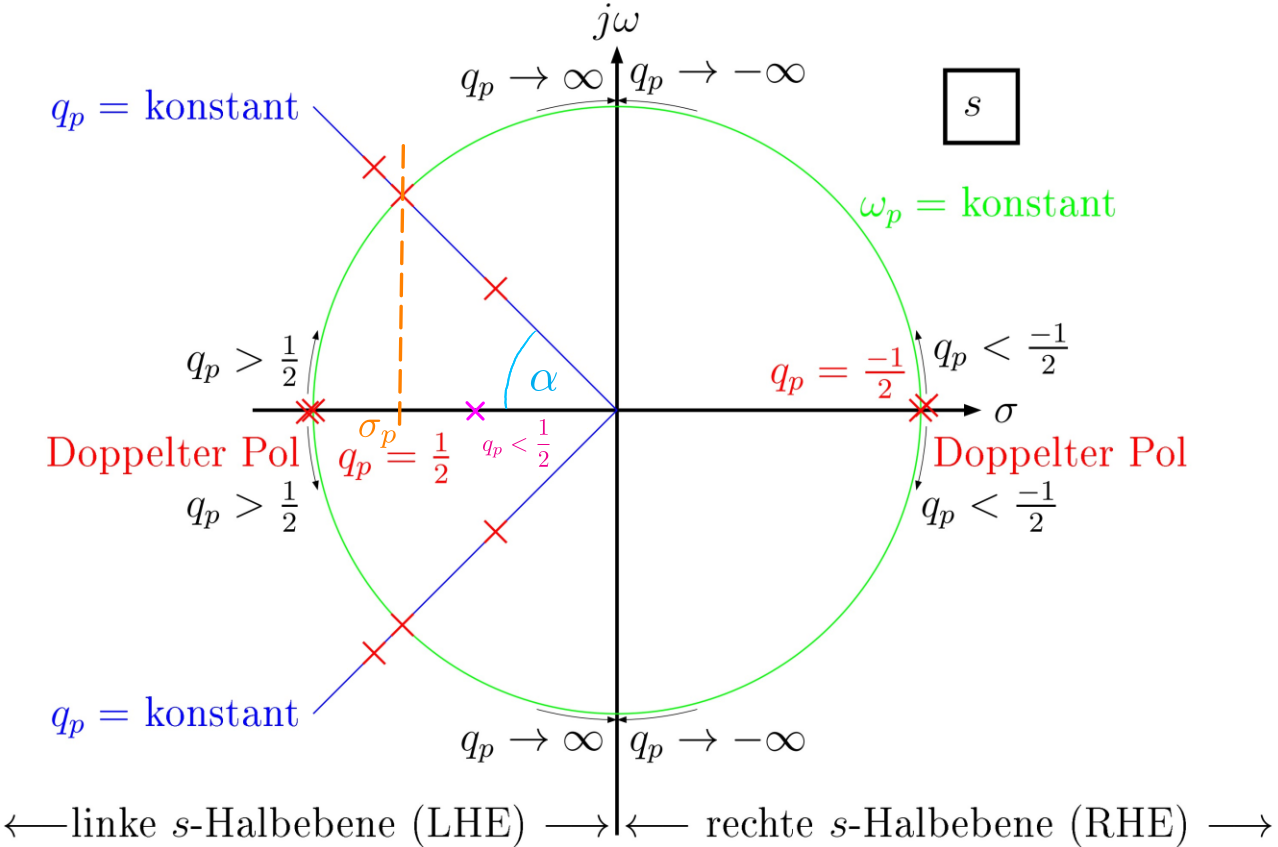
\includegraphics[width=\columnwidth]{images/pole_nullstellen_koeffizienten.png}
\end{minipage}
\hfill
\begin{minipage}[c]{0.42\columnwidth}
    \textbf{Hinweise}
    \begin{itemize}
        \item Pole sind als rote Kreuze dargestellt
        \item Für die NS (Nullstellenfrequenzen, Nullstellengüten) gelten die gleichen
            geometrischen Beziehungen wie für die Polstellen
    \end{itemize}
\end{minipage}






% next lecture (maybe):
% \subsection{Bestimmung Frequenzgang aus UTF}

% \subsection{Bestimmung Frequenzgang aus Pol-/ NS der UTF}



% \subsubsection{Umrechnung}

% $$ \boxed{ H(j \omega) = H(s) \Big|_{s = j \omega} = |H(j \omega)| \cdot e^{j \theta(\omega)} } $$


% \begin{tabular}{ll}
%     $H(s)$          & Übertragungsfunktion (UTF) \\\
%     $H(j \omega)$   & Frequenzgang \\
%     $|H(j \omega)|$ & Amplitudengang \\
%     $\theta(\omega)$& Phasengang
% \end{tabular}